\documentclass[UTF-8,twoside,cs4size]{ctexart}
\usepackage{amsmath}
\usepackage{amssymb}
\usepackage{geometry}
\usepackage{setspace}
\usepackage{xeCJK}
\usepackage{ulem}
\usepackage{pstricks}
\usepackage{pstricks-add}
\usepackage{bm}
\usepackage{mathtools}
\usepackage{breqn}
\usepackage{mathrsfs}
\usepackage{esint}
\usepackage{textcomp}
\usepackage{upgreek}
\usepackage{pifont}
\usepackage{tikz}
\usepackage{circuitikz}
\usepackage{caption}
\usepackage{xcolor}
\usepackage{tabularx}
\usepackage{array}
\usepackage{pgfplots}
\usepackage{multirow}

\newcolumntype{Y}{>{\centering\arraybackslash}X}
\geometry{a4paper,centering,top=0.75cm,bottom=2.54cm,left=2cm,right=2cm}
\pagestyle{plain}
\captionsetup{font=small}

\CTEXsetup[name={,.}]{section}
\CTEXsetup[format={\raggedright\bfseries\noindent\Large}]{section}
\CTEXsetup[format={\raggedright\bfseries\quad\large}]{subsection}
\CTEXsetup[format={\raggedright\bfseries\qquad}]{subsubsection}

\setstretch{1.5}

\setCJKfamilyfont{boldsong}[AutoFakeBold = {2.17}]{SimSun}
\newcommand*{\boldsong}{\CJKfamily{boldsong}}
\DeclareMathOperator\dif{d\!}

\begin{document}
	\begin{flushright}
		\zihao{2}{分组号:3-07}
	\end{flushright}
	
	\noindent{\zihao{-2}\boldsong\bfseries 《\,\, 基\,\, 础\,\, 物\,\, 理\,\, 实\,\, 验\,\, 》\,\, 实\,\, 验\,\, 报\,\, 告\,\, }
	
	\noindent\textit{实验名称\uline{\quad 微波布拉格衍射\qquad\qquad\qquad\,\qquad\qquad\qquad\qquad\qquad}指导教师\uline{\qquad\,\,\,易栖如\,\,\,\qquad}}
	
	\noindent\textit{姓\qquad 名\uline{\,\,\, 桂庭辉\,\,\,}\,学号\uline{\,\,\,{\upshape2019K8009929019}\,\,\,}\,专\qquad 业\uline{\,\,\,计算机科学与技术\,\,\,}\,班级\uline{\,\,\,\upshape{03}\,\,\,}\,座号\uline{\,\,\,\upshape{6}\,\,\,}}
	
	\noindent\textit{实验日期\uline{\,\,{\upshape 2020}\,\,}年\uline{\,\,{\upshape 11}\,\,}月\uline{\,\,{\upshape11}\,\,}日\,\,实验地点\uline{\,\,\,教学楼{\upshape717}\,\,\,}调课/补课\uline{\,\,\,$ \square $是\,\,\,}成绩评定\uline{\,\,\,\quad\qquad\qquad}}
	
	\begin{table}[h]
		\centering
		\psset{linewidth=2pt}
		\begin{pspicture}(-1,-0.1)(1,0.1)
		\psline(-9,0)(9,0)
		\end{pspicture}
	\end{table}

	\section{实验目的}
		1.了解与学习微波产生的基本原理以及传播和接收等基本特性;
		
		2.观测微波衍射、干涉等实验现象;
		
		3.观测模拟晶体的微波布拉格衍射现象;
		
		4.通过迈克尔逊实验观测微波波长。
		
	\section{实验器材}
		DHMS-1型微波光学综合实验仪一套,包括:X波段微波信号源、微波发生器、发射喇叭、接收喇叭、微波检波器、检波信号数字显示器、可旋转载物平台和支架,以及实验用附件(反射板、分束板、单缝板、双缝板、晶体模型、读数机构等)。
		
	\section{实验原理}
		微波波长从1\,m到0.1\,mm,其频率范围为$ 300\,\mathrm{MHz}\sim3000\,\mathrm{GHz} $,是无线电波中波长最短的电磁波。微波波长介于一般无线电波与光波之间,因此它不仅具有无线电波的性质,还具有光波的性质,即具有光的直线传播、反射、折射、衍射、干涉等性质。微波波长与普通电磁波相比要短得多,因此其反射、辐射、传播和接收器件都有自己的特殊性;同时,它的波长又比X射线、光波长得多,故而用微波来仿真“晶格”衍射,发生明显衍射效应的“晶格”可以放大到宏观的尺度。
		
		\subsection{微波的产生和接收}
		本次实验中所使用的微波发生器采用电调制方法实现。微波发生器内部有一个电压可调控制的VCO,用于产生一个$ 4.4\,\mathrm{GHz}\sim 5.2\,\mathrm{GHz} $的信号,它的输出频率可以随输入电压的不同作相应改变,经过滤波器后取二次谐波$ 8.8\,\mathrm{GHz}\sim9.8\,\mathrm{GHz} $,经过衰减器作适当的衰减后,再放大,经过隔离器后,通过探针输出至波导口,再通过E面天线发射出去。
		
		接收部分采用检波/数显一体化设计。由E面喇叭天线接收微波信号,传给高灵敏度的检波管后转化为电信号,通过穿心电容送出检波电压,再通过A/D转换(即模-数转换,Anglog-Digital),由液晶显示器显示微波相对强度。
		
		\subsection{微波的单缝衍射实验}
		当一平面微波入射到一宽度和微波波长可比拟的一狭缝时,在缝后会发生如光波一般的衍射现象,其示意图与强度分布如图\ref{fig-single}\,。
		
		\begin{figure}[h]
			\centering
			\begin{tikzpicture}
				\draw (-6.2,0)--(6.2,0);
				\draw (0,0)--(0,5);
				\node [below] at(-6,0) {$ \frac{-3a\sin\varphi}{\lambda} $};
				\node [below] at(-4,0) {$ \frac{-2a\sin\varphi}{\lambda} $};
				\node [below] at(-2,0) {$ \frac{-a\sin\varphi}{\lambda} $};
				\node [below] at(2,0) {$ \frac{a\sin\varphi}{\lambda} $};
				\node [below] at(4,0) {$ \frac{2a\sin\varphi}{\lambda} $};
				\node [below] at(6,0) {$ \frac{3a\sin\varphi}{\lambda} $};
				\node at(0,-0.5) {0};
				\draw [very thick,domain=-6:-0.01,samples=100] plot (\x,{5*pow(sin(\x*pi/2 r)/(\x*pi/2),2)});
				\draw [very thick,domain=0.01:6,samples=100] plot (\x,{5*pow(sin(\x*pi/2 r)/(\x*pi/2),2)});
				\draw [very thick] (0.01,5)--(-0.01,5);
				
				\draw (-10,2)--(-9.5,2)--(-9.5,1.8)--(-11,1.8)--(-11,2)--(-10,2);
				\draw (-8,2)--(-8.5,2)--(-8.5,1.8)--(-7,1.8)--(-7,2)--(-8,2);
				\draw [thick,<-] (-9.5,2)--(-9.5,4);
				\draw [thick,<-] (-8.5,2)--(-8.5,4);
				\draw [thick] (-9.5,2)--(-9.5,1.8);
				\draw [thick] (-8.5,2)--(-8.5,1.8);
				\draw [dashed] (-9.5,1.8)--(-9.5,-1);
				\draw [dashed] (-8.5,1.8)--(-8.5,-1);
				\draw [thick,->] (-9.5,1.8)--(-9,0);
				\draw [thick,->] (-8.5,1.8)--(-8,0);
				\draw [<->] (-9.5,-0.5)--(-8.5,-0.5);
				%\draw (-8.5,0.5) to[out=0,in=210]  (-8.16,0.6);
				\draw (-8.5,0.5) arc (270:285:1.3);
				
				\node [below] at(-9,-0.5) {$ a $};
				\node [below] at(-8.3,0.5) {$ \theta $};
			\end{tikzpicture}
			\caption{单缝衍射示意图与强度分布}
			\label{fig-single}
		\end{figure}
	
	如为一维衍射,微波单缝衍射图样的强度分布规律为
	\[I=I_0\frac{\sin^2\mu}{\mu^2}\qquad\left(\mu=\frac{\uppi a\sin\theta}{\lambda}\right)\]
	其中$ I_0 $为中央主极大中心的微波强度,$ a $为单缝的宽度,$ \lambda $是微波的波长,$ \theta $为衍射角。与光的单缝衍射一样,当$ a\sin\theta=\pm k\lambda\,(k=1,2,3,\cdots) $时,相应的$ \theta $角位置衍射强度为0。如测出衍射强度分布则可依据第一级衍射最小值所对应的$ \theta $,求出微波波长$ \lambda=a\sin\theta $.
	
	\subsection{微波的双缝干涉实验}
	当一平面波垂直入射到一金属板的两条狭缝上,狭缝就成为次级波波源。由两缝发出的次级波是相干波,因此在金属板的背后空间中,将产生干涉现象。由于波通过每个缝都有衍射现象,因此实验将是干涉与衍射两者结合的结果。为了只研究主要来自两缝中央衍射波相互干涉的结果,令双缝的缝宽$ a $接近$ \lambda $。当两缝之间的间隔$ b $较大时,干涉强度受单缝衍射的影响小;当$ b $较大时,干涉强度受单缝衍射影响大。干涉加强的角度为
	\[\varphi=\arcsin\left(\frac{k\lambda}{a+b}\right)\qquad k=1,2,3,\cdots\]
	干涉减弱的角度为
	\[\varphi=\arcsin\left(\frac{2k+1}{2}\cdot\frac{\lambda}{a+b}\right)\qquad k=1,2,3,\cdots\]
	
	\subsection{微波的迈克尔逊干涉实验}
	1881年物理学家迈克尔逊与莫雷合作,为研究“以太”漂移而设计制造了利用分振幅法产生双光束以实现干涉的迈克尔逊干涉仪。
	
	\begin{figure}[h]
		\centering
		\begin{tikzpicture}
			\draw (0,0.1)--(1,1.1)--(1.1,1)--(0,-0.1)--(-1,-1.1)--(-1.1,-1)--(0,0.1);
			\draw [thick] (0.3,0)--(4.3,0);
			\draw [thick] (-0.3,0)--(-4.3,0);
			\draw [thick,->] (-4.3,0)--(-2.3,0);
			\draw [thick,<->] (1.3,0)--(3.3,0);
			\node [below] at(2.3,0) {$ d_2 $};
			\draw [ultra thick] (4.5,-1)--(4.5,1);
			\node [below] at(4.5,-1) {反射镜B};
			\node [above left] at(0,0) {半透镜};
			\draw [thick] (0,-0.3)--(0,-3.3);
			\draw [thick,->] (0,-0.3)--(0,-2.3);
			\draw [thick] (0,0.3)--(0,3.3);
			\draw [thick,<->] (0,1.3)--(0,2.3);
			\node [left] at(0,1.8) {$ d_1 $};
			\node [below left] at(-0.1,0.1) {$ 45^{\circ} $};
			\draw [ultra thick] (-1,3.5)--(1,3.5);
			\node [above] at(0,3.5) {反射镜A};
			
			\draw (0,-3.3)--(0.5,-3.3)--(0.15,-4.3)--(0.5,-4.3)--(0.5,-4.7)--(-0.5,-4.7)--(-0.5,-4.3)--(-0.15,-4.3)--(-0.5,-3.3)--(0,-3.3);
			\node [below] at(0,-4.7) {接收喇叭};
			\draw (-4.3,0)--(-4.3,0.5)--(-5.3,0.15)--(-5.3,0.5)--(-5.7,0.5)--(-5.7,-0.5)--(-5.3,-0.5)--(-5.3,-0.15)--(-4.3,-0.5)--(-4.3,0);
			\node [below] at(-5,-0.5) {发射喇叭};
		\end{tikzpicture}
		\caption{迈克尔逊干涉原理示意图}
		\label{fig-double}
	\end{figure}

	在微波前进的方向上放置一个与波传播方向成$ 45^{\circ} $角的半透射半反射的分束板将入射波分成一束向金属板A传播,另一束向金属板B传播。由于A、B金属板全反射,两列波再回到半透射半反射的分束板,会合后到达微波接收器处。这两束微波频率相同,在接收器处将发生干涉,干涉叠加的强度由两束波的光程差(即相位差)决定。
	
	当两波的相位差为$ 2k\uppi\;(k=\pm1,\pm2,\pm3,\cdots) $时,干涉最强;当两波相位差为$ (2k+1)\uppi $时,则干涉最弱。固定A、B中其中一块板,另一块板可以沿着微波传播方向前后移动。当微波接收信号从极小(或极大)值到第$ n+1 $次极小(或极大)值,反射板移动距离为$ L $,则微波波长$ \lambda=\frac{2L}{n} $。
	
	\subsection{微波布拉格衍射}
		\subsubsection{晶体结构}
		组成晶体的原子或分子会按一定规律在空间内周期性排列。其中最简单的结构,是组成晶体的原子在直角坐标中沿$ x,y,z $三个方向,按固定的距离$ a $(晶格常数)在空间依序重复排列,形成简单的立方点阵。
		
		\begin{figure}[h]
			\centering
			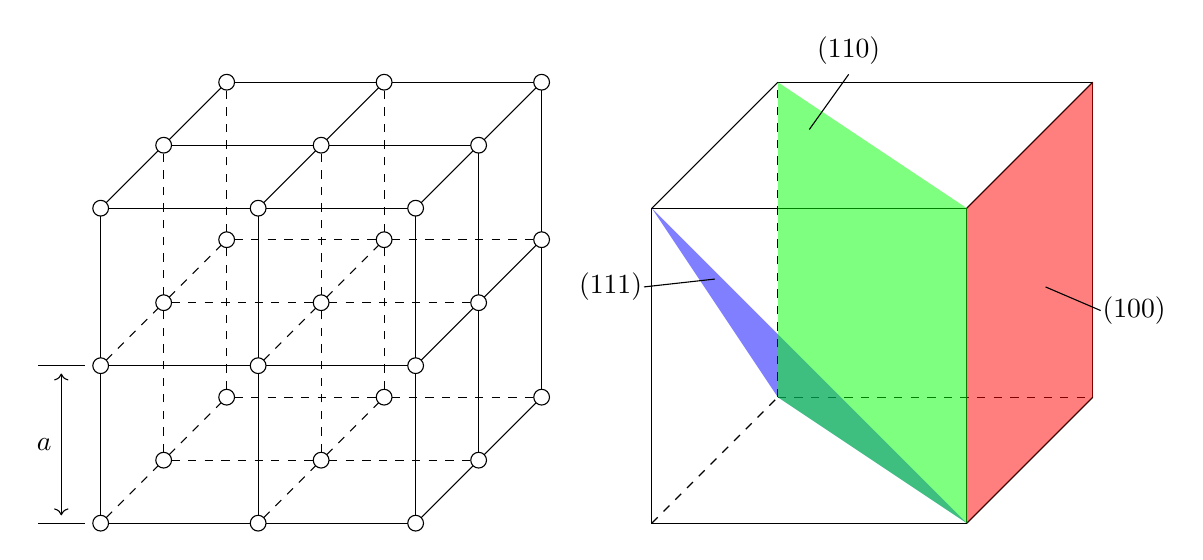
\begin{tikzpicture}
				\draw (0,0) circle [radius=0.1];
				\draw (2,0) circle [radius=0.1];
				\draw (4,0) circle [radius=0.1];
				\draw (4,2) circle [radius=0.1];
				\draw (4,4) circle [radius=0.1];
				\draw (0,2) circle [radius=0.1];
				\draw (0,4) circle [radius=0.1];
				\draw (2,2) circle [radius=0.1];
				\draw (2,4) circle [radius=0.1];
				\draw (0.8,0.8) circle [radius=0.1];
				\draw (0.8,2.8) circle [radius=0.1];
				\draw (0.8,4.8) circle [radius=0.1];
				\draw (2.8,0.8) circle [radius=0.1];
				\draw (4.8,0.8) circle [radius=0.1];
				\draw (2.8,2.8) circle [radius=0.1];
				\draw (2.8,4.8) circle [radius=0.1];
				\draw (4.8,2.8) circle [radius=0.1];
				\draw (4.8,4.8) circle [radius=0.1];				
				\draw (1.6,1.6) circle [radius=0.1];				
				\draw (3.6,1.6) circle [radius=0.1];				
				\draw (5.6,1.6) circle [radius=0.1];				
				\draw (1.6,3.6) circle [radius=0.1];				
				\draw (1.6,5.6) circle [radius=0.1];				
				\draw (3.6,3.6) circle [radius=0.1];				
				\draw (3.6,5.6) circle [radius=0.1];				
				\draw (5.6,3.6) circle [radius=0.1];				
				\draw (5.6,5.6) circle [radius=0.1];
				
				\draw (0.1,0)--(1.9,0);
				\draw (0,0.1)--(0,1.9);
				\draw (0,2.1)--(0,3.9);
				\draw (2.1,0)--(3.9,0);
				\draw (0.1,2)--(1.9,2);
				\draw (0.1,4)--(1.9,4);
				\draw (2.1,2)--(3.9,2);
				\draw (2.1,4)--(3.9,4);
				\draw (2,0.1)--(2,1.9);
				\draw (4,0.1)--(4,1.9);
				\draw (2,2.1)--(2,3.9);
				\draw (4,2.1)--(4,3.9);
				\draw [dashed] (0.8,0.9)--(0.8,2.7);
				\draw [dashed] (2.8,0.9)--(2.8,2.7);
				\draw (4.8,0.9)--(4.8,2.7);
				\draw [dashed] (0.9,0.8)--(2.7,0.8);
				\draw [dashed] (0.9,2.8)--(2.7,2.8);
				\draw (0.9,4.8)--(2.7,4.8);
				\draw [dashed] (0.8,2.9)--(0.8,4.7);
				\draw [dashed] (2.8,2.9)--(2.8,4.7);
				\draw (4.8,2.9)--(4.8,4.7);
				\draw [dashed] (2.9,0.8)--(4.7,0.8);
				\draw [dashed] (2.9,2.8)--(4.7,2.8);
				\draw (2.9,4.8)--(4.7,4.8);
				\draw [dashed] (1.6,1.7)--(1.6,3.5);
				\draw [dashed] (3.6,1.7)--(3.6,3.5);
				\draw (5.6,1.7)--(5.6,3.5);
				\draw [dashed] (1.6,3.7)--(1.6,5.5);
				\draw [dashed] (3.6,3.7)--(3.6,5.5);
				\draw (5.6,3.7)--(5.6,5.5);
				\draw [dashed] (1.7,1.6)--(3.5,1.6);
				\draw [dashed] (1.7,3.6)--(3.5,3.6);
				\draw (1.7,5.6)--(3.5,5.6);
				\draw [dashed] (3.7,1.6)--(5.5,1.6);
				\draw [dashed] (3.7,3.6)--(5.5,3.6);
				\draw (3.7,5.6)--(5.5,5.6);				
				\draw [dashed] (0.07,0.07)--(0.73,0.73);
				\draw [dashed] (0.07,2.07)--(0.73,2.73);
				\draw (0.07,4.07)--(0.73,4.73);				
				\draw [dashed] (2.07,0.07)--(2.73,0.73);
				\draw [dashed] (2.07,2.07)--(2.73,2.73);
				\draw (2.07,4.07)--(2.73,4.73);				
				\draw (4.07,0.07)--(4.73,0.73);
				\draw (4.07,2.07)--(4.73,2.73);
				\draw (4.07,4.07)--(4.73,4.73);				
				\draw [dashed] (0.87,0.87)--(1.53,1.53);
				\draw [dashed] (0.87,2.87)--(1.53,3.53);
				\draw (0.87,4.87)--(1.53,5.53);				
				\draw [dashed] (2.87,0.87)--(3.53,1.53);
				\draw [dashed] (2.87,2.87)--(3.53,3.53);
				\draw (2.87,4.87)--(3.53,5.53);				
				\draw (4.87,0.87)--(5.53,1.53);
				\draw (4.87,2.87)--(5.53,3.53);
				\draw (4.87,4.87)--(5.53,5.53);
				\draw (-0.2,0)--(-0.8,0);				
				\draw (-0.2,2)--(-0.8,2);
				\draw [<->](-0.5,0.1)--(-0.5,1.9);
				\node [left] at(-0.5,1) {$ a $};
				
				\draw (7,0) rectangle (11,4);
				\draw (7,4)--(8.6,5.6);
				\draw (11,4)--(12.6,5.6);
				\draw (8.6,5.6)--(12.6,5.6);
				\draw (11,0)--(12.6,1.6);
				\draw (12.6,1.6)--(12.6,5.6);
				\draw [dashed] (7,0)--(8.6,1.6);
				\draw [dashed] (8.6,1.6)--(8.6,5.6);
				\draw [dashed] (8.6,1.6)--(12.6,1.6);
				\fill [blue,fill opacity=0.5] (8.6,1.6)--(7,4)--(11,0)--(8.6,1.6)--cycle;
				\fill [green,fill opacity=0.5] (8.6,1.6)--(8.6,5.6)--(11,4)--(11,0)--cycle;
				\fill [red,fill opacity=0.5] (11,0)--(12.6,1.6)--(12.6,5.6)--(11,4)--(11,0)--cycle;
				\draw (6.9,3)--(7.8,3.1);
				\node [left] at(7,3) {(111)};
				\draw (9,5)--(9.5,5.7);
				\node [above] at(9.5,5.7) {(110)};
				\draw (12,3)--(12.7,2.7);
				\node [right] at(12.6,2.7) {(100)};
			\end{tikzpicture}
			\caption{立方晶格模型与晶面指数}
			\label{fig-JingGe}
		\end{figure}
	
		组成晶体的原子可以看成分别作处在一系列相互平行而且间距一定的平面族上,这些平面称为晶面。在晶面的不同取法中,最重要且最常用的三种即为图\ref{fig-JingGe}\,中的(111)面、(110)面、(100)面,圆括号中的三个数字称为晶面指数。晶面指数的一般取法为:在右手系下取平面在$ x,y,z $轴上的截距$ x_0,y_0,z_0 $,取其倒数之比$ \frac1{x_0}:\frac1{y_0}:\frac1{z_0} $,将其化为最小整数比$ x_1:y_1:z_1 $,则该平面的晶面指数为$ (x_1y_1z_1) $。一般而言,晶面指数为$ (n_1n_2n_3) $的晶面族,其相邻的两个晶面间距$ d=\frac{a}{\sqrt{n_1^2+n_2^2+n_3^2}} $.
		
		\subsubsection{布拉格衍射}
		
		类似光波入射到二维的平面光栅要受到光栅的衍射,电磁波入射到晶体也要受到晶体的衍射。用三维空间中原子组成的格点取代平面上的小孔,可看作是一个三维的光栅网络。晶体对电子波衍射的实质是每个格点上的原子产生的散射波的相干叠加。它们的相干叠加的第一步可看作是统一晶面上各个原子发出的散射波的相干叠加,形成每一个晶面的衍射波;第二步是同一晶面族的不同晶面的衍射波之间的相干叠加。
		
		\begin{figure}[h]
			\centering
			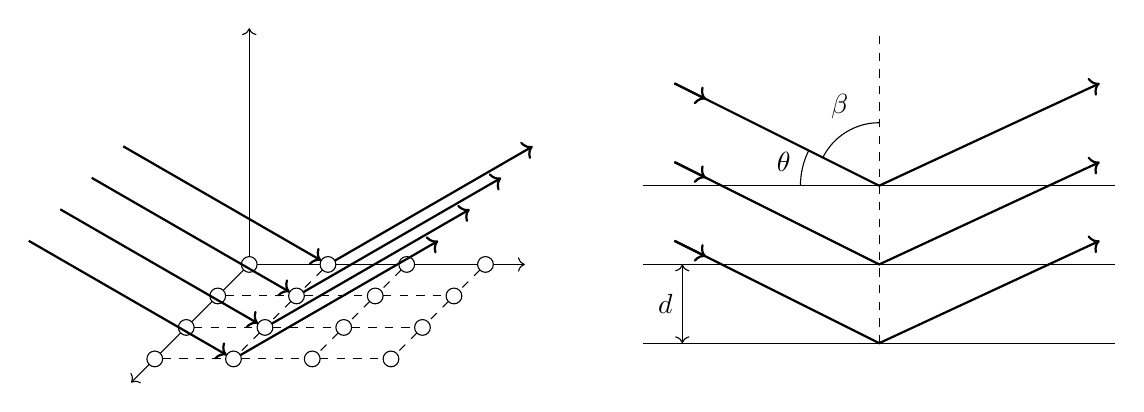
\begin{tikzpicture}
				\draw (-3,0)--(3,0);
				\draw (-3,2)--(3,2);
				\draw (-3,1)--(3,1);
				\draw [dashed] (0,0)--(0,4);
				\draw [<->] (-2.5,0)--(-2.5,1);
				\node [left] at(-2.5,0.5) {$ d $};
				\draw [thick,->] (-2.6,1.3)--(0,0)--(2.8,1.3);
				\draw [thick,->] (-2.6,1.3)--(-2.2,1.1);
				\draw [thick,->] (-2.6,2.3)--(0,1)--(2.8,2.3);
				\draw [thick,->] (-2.6,2.3)--(-2.2,2.1);
				\draw [thick,->] (-2.6,3.3)--(0,2)--(2.8,3.3);
				\draw [thick,->] (-2.6,3.3)--(-2.2,3.1);
				\draw (-1,2) arc (180:154:1);
				\draw (0,2.8) arc (90:154:0.8);
				\node [left] at(-1,2.3) {$\theta$};
				\node at(-0.5,3) {$\beta$};
				
				\draw (-8,1) circle [radius=0.1];
				\draw (-7,1) circle [radius=0.1];
				\draw (-6,1) circle [radius=0.1];
				\draw (-5,1) circle [radius=0.1];
				\draw (-8.4,0.6) circle [radius=0.1];
				\draw (-7.4,0.6) circle [radius=0.1];
				\draw (-6.4,0.6) circle [radius=0.1];
				\draw (-5.4,0.6) circle [radius=0.1];
				\draw (-8.8,0.2) circle [radius=0.1];
				\draw (-7.8,0.2) circle [radius=0.1];
				\draw (-6.8,0.2) circle [radius=0.1];
				\draw (-5.8,0.2) circle [radius=0.1];
				\draw (-9.2,-0.2) circle [radius=0.1];
				\draw (-7.2,-0.2) circle [radius=0.1];
				\draw (-8.2,-0.2) circle [radius=0.1];
				\draw (-6.2,-0.2) circle [radius=0.1];
				\draw [->] (-8,1.1)--(-8,4);
				\draw (-8.07,0.93)--(-8.33,0.67);
				\draw (-8.47,0.53)--(-8.73,0.27);
				\draw (-8.87,0.13)--(-9.13,-0.13);
				\draw [->] (-9.27,-0.27)--(-9.5,-0.5);
				\draw [dashed] (-7.07,0.93)--(-7.33,0.67);
				\draw [dashed] (-7.47,0.53)--(-7.73,0.27);
				\draw [dashed] (-7.87,0.13)--(-8.13,-0.13);
				\draw [dashed] (-6.07,0.93)--(-6.33,0.67);
				\draw [dashed] (-6.47,0.53)--(-6.73,0.27);
				\draw [dashed] (-6.87,0.13)--(-7.13,-0.13);
				\draw [dashed] (-5.07,0.93)--(-5.33,0.67);
				\draw [dashed] (-5.47,0.53)--(-5.73,0.27);
				\draw [dashed] (-5.87,0.13)--(-6.13,-0.13);
				\draw (-7.9,1)--(-7.1,1);
				\draw (-6.9,1)--(-6.1,1);
				\draw (-5.9,1)--(-5.1,1);
				\draw [->] (-4.9,1)--(-4.5,1);
				\draw [dashed] (-8.3,0.6)--(-7.5,0.6);
				\draw [dashed] (-7.3,0.6)--(-6.5,0.6);
				\draw [dashed] (-6.3,0.6)--(-5.5,0.6);
				\draw [dashed] (-8.7,0.2)--(-7.9,0.2);
				\draw [dashed] (-7.7,0.2)--(-6.9,0.2);
				\draw [dashed] (-6.7,0.2)--(-5.9,0.2);
				\draw [dashed] (-9.1,-0.2)--(-8.3,-0.2);
				\draw [dashed] (-8.1,-0.2)--(-7.3,-0.2);
				\draw [dashed] (-7.1,-0.2)--(-6.3,-0.2);
				\draw [thick,->] (-9.60,2.5)--(-7.086,1.05);
				\draw [thick,->] (-10.0,2.1)--(-7.486,0.65);
				\draw [thick,->] (-10.40,1.7)--(-7.886,0.25);
				\draw [thick,->] (-10.80,1.3)--(-8.286,-0.15);
				\draw [thick,->] (-6.91,1.05)--(-4.40,2.5);
				\draw [thick,->] (-7.31,0.65)--(-4.80,2.1);
				\draw [thick,->] (-7.71,0.25)--(-5.20,1.7);
				\draw [thick,->] (-8.11,-0.15)--(-5.60,1.3);
			\end{tikzpicture}
			\caption{同一晶面与不同晶面的散射波示意图}
			\label{fig-scatt}
		\end{figure}
	
		处在同一平面上的原子组成一个晶面,它们的散射波相干叠加的结果遵从反射定律。而从间隔为$ d $的相邻两个晶面反射的两束波的程差为$ 2d\sin\theta $,$ \theta $为入射角与晶面的夹角。显然只有满足
		\[2d\sin\theta=k\lambda,\qquad k=1,2,3,\cdots\]
		才能形成干涉极大。上式称为晶体衍射的布拉格条件,如果改用常用的入射角$ \beta $表示,则布拉格条件可改写为
		\[2d\cos\beta=k\lambda,\qquad k=1,2,3,\cdots\]
		在本次实验中,已知晶面间距$ d $,通过测量衍射极大时的入射角$ \beta $以求得波长$\lambda$.
		
		由于不同晶面族的曲线不同,晶面间隔也不同,因此当入射波方向及波长固定、晶体取向固定时,不同取向的晶面不能同时满足布拉格条件,甚至没有一族晶面能够满足布拉格条件。为了观察到尽可能多的衍射极大,得到尽可能多的关于晶体结构的信息,在研究晶体结构的实际工作中,采用不同的方法:转动晶体、采用多晶或粉末样品代替单晶、采用包含波长连续变化的X射线代替单一波长的X射线。在本实验中使用入射方向固定、波长单一的微波及单晶模型,从而采用转动晶体模型和接收喇叭的方向来进行对不同晶面的研究。
		
		~\
		
	\section{实验内容}
	四实验中所用微波频率一致,均为9.4\,GHz,打开电源后将微波频率设置为9.4\,GHz,并调整实验仪器在桌面上的位置与角度,使得检波器扫描范围能达到$ \pm50^\circ $。
	
	\subsection{实验1:微波的单缝衍射}
	转动接收臂使其指针指向载物台的$ 0^\circ $刻线,打开振荡器的电源,转动载物台,使其上的$ 180^\circ $刻线与发射臂的指针一致,调节发生器与接受器姿态,使其正对,微调接收喇叭的朝向,使得在$ \pm20^\circ $处的差异在2\,mV以内。
	
	调节衰减器,使二者正对时接收电表的指示在150\,mV左右。
	
	仪器安装时,按需要先调整单缝衍射板的缝宽,然后把单缝衍射板放到载物台,并使狭缝所在平面与入射方向垂直(微调狭缝角度使得当正对发生器的接收电表示数极大),把单缝的底座固定在载物台上。
	
	转动接收臂,在$ -40^\circ\sim40^\circ $内每隔$ 2^\circ $记下一次接收信号的大小。
	
	为了准确测量波长,需仔细寻找衍射极小的位置。在衍射极小附近,以$ 1^\circ $为步长精扫接收信号的变化。可把衰减器向零处旋转,以增大发射信号的强度,进而提高测量的灵敏度。
	
	根据记录数据,画出单缝衍射强度与衍射角度的关系曲线。并根据微波衍射强度一级极小角度$ \varphi $和缝宽$a$,计算微波波长$\lambda$和其百分误差。
	
	\subsection{实验2:微波的双缝干涉}
	放置双缝前,与实验1一样进行实验仪对准确认,使得发生器、接收器分别于$ 180^\circ,0^\circ $处正对,接收信号在$ \pm20^\circ $处强度相当。调节微波发射功率使得在零级极大处接收信号强度在150\,mV左右。
		
	按要求调整双缝干涉板的缝宽均为3.5\,cm。将双缝缝干射板安置在支座上时,应使双缝板平面与载物圆台上$ 90^\circ $指示线一致。在$ -50^\circ\sim50^\circ $范围内,每改变$ 2^\circ $读取一次液晶显示器的读数,并记录下来,然后就可以画出双缝干涉强度与角度的关系曲线。
	
	在两侧零级极大、零级极小、一级极小处以$ 1^\circ $为步长进行精扫,绘制精扫结果图象以确定极值点。
	
	根据微波干涉强度零级极大、零级极小、一级极大角度和缝宽$a$、缝间间隔$ b $,计算微波波长$\lambda$和其百分误差。
	
	\subsection{实验3:迈克尔逊干涉实验}
	根据微波的前进方向设置迈克尔逊干涉仪,在极大位置适当调节微波发生功率使其大于100\,mV,便于观察接收信号强度的变化与极小值。将可移动反射板装在一旋转读数机构上后,然后移动旋转读数机构上的手柄,使得可移动反射板移动,测出$ n+1 $个微波极小值,并同时从读数机构上读出可移反射板的移动距离$ L $,则波长满足$ \lambda=\frac{2L}{n} $。
	
	\subsection{实验4:布拉格衍射}
	同此前的实验一样,实验进行前需检查发生器和检波器的正对情况。
	\subsubsection{(100)晶面}
	将发生器与检波器正对,调节微波发生功率使得接收信号为$ 150\,\mathrm{mV} $左右。安装模型晶体,转动载物圆盘使得发生器位于$ -30^\circ $(即$ 330^\circ $)处,转动接收器使其位于$ 30^\circ $处,即使得入射角与探测方向相对晶面法线对称。将入射角在$ 30^\circ\sim80^\circ $范围内以$ 2^\circ $为步长步进,在相应的探测位置读得并记录接收信号强度。绘制入射角与接收信号强度间的图象。
	
	在信号强度极大值点附近以$ 1^\circ $为步长进行精扫,以确定极大值点对应的入射角。进而求得微波波长$ \lambda=2d\cos\beta $并计算百分误差。
	
	\subsubsection{(110)晶面}
	大致步骤与(100)晶面时一致,不同在于(100)晶面的晶面法线方向为载物圆盘上$ 0^\circ $方向,而(110)晶面的晶面法线方向为载物圆盘上$ 45^\circ $方向。此外粗扫时入射角范围调整为$ 30^\circ\sim70^\circ $,精扫时由于接收信号较弱可适当调节微波发生功率。
	
	\section{实验结果与数据处理}
	\subsection{实验1:微波的单缝衍射}
	测得的实验数据如下表
	\begin{table}[!h]
		\centering
		{\small(a)粗扫数据记录}\\
		\begin{tabularx}{\textwidth}{|c|Y|Y|Y|Y|Y|Y|Y|Y|Y|}
			\hline
			$ {\theta}\;(^\circ) $ & $ \bm 0 $ & $ \bm 2 $ & $ \bm 4 $ & $ \bm 6 $ & $ \bm 8 $ & $ \bm{10} $ & $ \bm{12} $ & $ \bm{14} $ & $ \bm{16} $\\
			\hline
			$ {U_{\theta+}}\;(\mathrm{mV}) $ & 100.1 & 92.8 & 69.2 & 60.3 & 59.6 & 52.7 & 26.0 & 14.8 & 5.1\\
			\hline
			$ U_{\theta-}\;(\mathrm{mV}) $ & 100.1 & 97.3 & 90.1 & 75.8 & 52.3 & 30.3 & 20.2 & 12.7 & 3.6\\
			\hline
			$ {\theta}\;(^\circ) $ & $ \bm{18} $ & $ \bm{20} $ & $ \bm{22} $ & $ \bm{24} $ & $ \bm{26} $ & $ \bm{28} $ & $ \bm{30} $ & $ \bm{32} $ & $ \bm{34} $\\
			\hline
			$ {U_{\theta+}}\;(\mathrm{mV}) $ & 2.1 & 0.4 & 0.0 & 0.0 & 0.0 & 0.0 & 0.0 & 0.3 & 0.8\\
			\hline
			$ U_{\theta-}\;(\mathrm{mV}) $ & 0.8 & 0.1 & 0.0 & 0.0 & 0.0 & 0.0 & 0.5 & 0.1 & 0.4\\
			\hline
			$ \theta\;(^\circ) $ & $ \bm{36} $ & $ \bm{38} $ & $ \bm{40} $ &&&&&&\\
			\hline
			$ {U_{\theta+}}\;(\mathrm{mV}) $ & 0.5 & 0.0 & 0.1 &&&&&& \\
			\hline
			$ U_{\theta-}\;(\mathrm{mV}) $ & 0.1 & 0.0 & 0.4 &&&&&& \\
			\hline
		\end{tabularx}
	
		{\small(b)正负侧极小值点附近细扫数据记录}\\
		\begin{tabularx}{\textwidth}{|c|Y|Y|Y|Y|Y|Y|Y|Y|Y|Y|Y|}
			\hline
			$ {\theta}\;(^\circ) $ & $ \bm{21} $ & $ \bm{22} $ & $ \bm{23} $ & $ \bm{24} $ & $ \bm{25} $ & $ \bm{26} $ & $ \bm{27} $ & $ \bm{28} $ & $ \bm{29} $ & $ \bm{30} $ & $ \bm{31} $\\
			\hline
			$ U_{\theta+}\;(\mathrm{mV}) $ & 0.4 & 0.0 & 0.0 & 0.1 & 0.3 & 0.4 & 0.2 & 0.2 & 0.1 & 0.5 & 2.1\\
			\hline
			$ {\theta}\;(^\circ) $ & $ \bm{21} $ & $ \bm{22} $ & $ \bm{23} $ & $ \bm{24} $ & $ \bm{25} $ & $ \bm{26} $ & $ \bm{27} $ & $ \bm{28} $ & $ \bm{29} $ &  & \\
			\hline
			$ U_{\theta-}\;(\mathrm{mV}) $ & 0.2 & 0.0 & 0.1 & 0.3 & 0.3 & 0.4 & 0.3 & 0.5 & 1.7 &  & \\
			\hline
		\end{tabularx}
		\caption{单缝衍射数据记录表}
	\end{table}

	根据表中数据可分别作出粗扫下的$ \theta-U $图象、细扫下两个极小值点附近的$ \theta-U $图象:
	
	\begin{figure}[!h]
		\centering
		\begin{tikzpicture}			
			\begin{axis}[
				width=10cm,height=6cm,
				title={\small (a)\;单缝衍射粗扫结果图},
				xlabel=$ \theta\;(^\circ) $,ylabel=$ U\;(\mathrm{mV}) $,
				xmin=-50,xmax=50,
				ymin=0,ymax=110,
				xtick={-50,-40,-30,-20,-10,-0,10,20,30,40,50},
				ytick={0,10,20,30,40,50,60,70,80,90,100,110},
				grid style=dashed,
				ymajorgrids=true,
				xmajorgrids=true,
				]
				\addplot [thick,mark=+,smooth] coordinates {
				(-40,0.4)(-38,0.0)(-36,0.1)(-34,0.4)(-32,0.1)
				(-30,0.5)(-28,0.0)(-26,0)(-24,0)(-22,0)
				(-20,0.1)(-18,0.8)(-16,3.6)(-14,12.7)(-12,20.2)
				(-10,30.3)(-8,52.3)(-6,75.8)(-4,90.1)(-2,97.3)
				(0,100.1)
				(2,92.8)(4,69.2)(6,60.3)(8,59.6)(10,52.7)
				(12,26.0)(14,14.8)(16,5.1)(18,2.1)(20,0.4)
				(22,0)(24,0)(26,0)(28,0)(30,0.5)
				(32,0.1)(34,0.4)(36,0.1)(38,0)(40,0.4)
			};
			\end{axis}
		\end{tikzpicture}
	\\
		\begin{tikzpicture}
			\begin{axis}[
				width=6cm,height=5cm,
				title={\small (b)\;单缝衍射正侧极小值处细扫图},		
				xlabel=$ \theta\;(^\circ) $,ylabel=$ U\;(\mathrm{mV}) $,
				xmin=20,xmax=32,
				ymin=0,ymax=2.5,
				xtick={20,22,24,26,28,30,32},
				ytick={0,0.5,1,1.5,2,2.5},
				grid style=dashed,
				ymajorgrids=true,
				xmajorgrids=true,
				]
				\addplot [thick,mark=+,smooth] coordinates {
					(21,0.4)(22,0)(23,0)(24,0.1)(25,0.3)(26,0.4)
					(27,0.2)(28,0.2)(29,0.1)(30,0.5)(31,2.1)
				};
			\end{axis}
		\end{tikzpicture}
	\qquad
	\begin{tikzpicture}
	\begin{axis}[
		width=6cm,height=5cm,
		title={\small (c)\;单缝衍射负侧极小值处细扫图},		
		xlabel=$ \theta\;(^\circ) $,ylabel=$ U\;(\mathrm{mV}) $,
		xmin=-30,xmax=-20,
		ymin=0,ymax=2.5,
		xtick={-20,-22,-24,-26,-28,-30},
		ytick={0,0.5,1,1.5,2,2.5},
		grid style=dashed,
		ymajorgrids=true,
		xmajorgrids=true,
		]
		\addplot [thick,mark=+,smooth] coordinates {
			(-21,0.2)(-22,0)(-23,0.1)(-24,0.3)
			(-25,0.3)
			(-26,0.4)(-27,0.3)(-28,0.5)(-29,1.7)
		};
	\end{axis}
	\end{tikzpicture}
	\captionsetup{skip=0pt}
	\caption{单缝衍射实验结果图}
	\end{figure}

	根据细扫图7-(b,c)的结果,可以估算得到$ \theta=22.25^\circ $,代入计算可得\[ \lambda=a\sin\theta=3.0292\,\mathrm{cm} \]误差率为$ 5.09\% $.
	
	\subsection{实验2:微波的双缝干涉}
	测得实验数据如下表:
	
	\begin{table}[!h]
		\centering
		{\small(a)粗扫数据记录}
		\begin{tabularx}{\textwidth}{|c|Y|Y|Y|Y|Y|Y|Y|Y|Y|}
			\hline
			$ {\theta}\;(^\circ) $ & $ \bm 0 $ & $ \bm 2 $ & $ \bm 4 $ & $ \bm 6 $ & $ \bm 8 $ & $ \bm{10} $ & $ \bm{12} $ & $ \bm{14} $ & $ \bm{16} $\\
			\hline
			$ {U_{\theta+}}\;(\mathrm{mV}) $ & 36.1 & 35.8 & 21.7 & 4.3 & 0.8 & 0.1 & 0.0 & 1.2 & 3.6\\
			\hline
			$ U_{\theta-}\;(\mathrm{mV}) $ & 36.1 & 31.2 & 24.1 & 13.2 & 2.0 & 0.1 & 0.3 & 1.3 & 5.9\\
			\hline
			$ {\theta}\;(^\circ) $ & $ \bm{18} $ & $ \bm{20} $ & $ \bm{22} $ & $ \bm{24} $ & $ \bm{26} $ & $ \bm{28} $ & $ \bm{30} $ & $ \bm{32} $ & $ \bm{34} $\\
			\hline
			$ {U_{\theta+}}\;(\mathrm{mV}) $ & 6.9 & 17.5 & 23.7 & 19.8 & 4.2 & 2.0 & 0.9 & 0.7 & 0.5\\
			\hline
			$ U_{\theta-}\;(\mathrm{mV}) $ & 13.5 & 18.6 & 22.5 & 13.6 & 4.5 & 1.8 & 1.0 & 0.6 & 0.7\\
			\hline
			$ \theta\;(^\circ) $ & $ \bm{36} $ & $ \bm{38} $ & $ \bm{40} $ & $ \bm{42} $ & $ \bm{44} $ & $ \bm{46} $ & $ \bm{48} $ & $ \bm{50} $ &\\
			\hline
			$ {U_{\theta+}}\;(\mathrm{mV}) $ & 0.9 & 1.5 & 1.2 & 0.3 & 0.5 & 2.6 & 4.5 & 3.1 & \\
			\hline
			$ U_{\theta-}\;(\mathrm{mV}) $ & 1.6 & 1.5 & 0.7 & 0.2 & 1.3 & 4.6 & 3.5 & 1.2 & \\
			\hline
		\end{tabularx}
	
		~\
		
		{\small(b)正负侧一级极大处细扫数据}\\
		\begin{tabularx}{\textwidth}{|c|c|Y|Y|Y|Y|Y|Y|Y|Y|Y|}
			\hline
			\multirow{4}*{一级极大} & $ \theta\;(^\circ) $ & $ \bm{18} $ & $ \bm{19} $ & $ \bm{20} $ & $ \bm{21} $ & $ \bm{22} $ & $ \bm{23} $ & $ \bm{24} $ & $ \bm{25} $ & $ \bm{26} $\\
			\cline{2-11}
			& $ U_{\theta+}\;(\mathrm{mV}) $ & 7.0 & 10.2 & 16.4 & 21.0 & 23.6 & 22.9 & 18.6 & 13.6 & 7.4\\
			\cline{2-11}
			& $ \theta\;(^\circ) $ & $ \bm{18} $ & $ \bm{19} $ & $ \bm{20} $ & $ \bm{21} $ & $ \bm{22} $ & $ \bm{23} $ & $ \bm{24} $ & $ \bm{25} $ & $ \bm{26} $\\
			\cline{2-11}
			& $ U_{\theta-}\;(\mathrm{mV}) $ & 13.1 & 16.0 & 19.3 & 21.7 & 22.1 & 18.8 & 13.6 & 7.1 & 4.4\\
			\hline
		\end{tabularx}
				
		~\
		
		{\small(c)正负侧零级极小处细扫数据}\\
		\begin{tabularx}{\textwidth}{|c|c|Y|Y|Y|Y|Y|Y|Y|Y|Y|}
			\hline
			\multirow{4}*{零级极小} & $ \theta\;(^\circ) $ & $ \bm{7} $ & $ \bm{8} $ & $ \bm{9} $ & $ \bm{10} $ & $ \bm{11} $ & $ \bm{12} $ & $ \bm{13} $ & $ \bm{14} $ & $ \bm{15} $\\
			\cline{2-11}
			& $ U_{\theta+}\;(\mathrm{mV}) $ & 1.4 & 0.7 & 0.3 & 0.1 & 0.0 & 0.0 & 0.3 & 1.0 & 2.5\\
			\cline{2-11}
			& $ \theta\;(^\circ) $ & $ \bm{7} $ & $ \bm{8} $ & $ \bm{9} $ & $ \bm{10} $ & $ \bm{11} $ & $ \bm{12} $ & $ \bm{13} $ & $ \bm{14} $ & $ \bm{15} $\\
			\cline{2-11}
			& $ U_{\theta-}\;(\mathrm{mV}) $ & 3.7 & 1.3 & 0.4 & 0.1 & 0.1 & 0.2 & 0.6 & 1.0 & 2.2\\
			\hline
		\end{tabularx}
		
		~\
		
		{\small(d)正负侧一级极小处细扫数据}\\
		\begin{tabularx}{\textwidth}{|c|c|Y|Y|Y|Y|Y|Y|Y|Y|Y|}
			\hline
			\multirow{4}*{一级极小} & $ \theta\;(^\circ) $ & $ \bm{29} $ & $ \bm{30} $ & $ \bm{31} $ & $ \bm{32} $ & $ \bm{33} $ & $ \bm{34} $ & $ \bm{35} $ & $ \bm{36} $ & $ \bm{37} $\\
			\cline{2-11}
			& $ U_{\theta+}\;(\mathrm{mV}) $ & 1.3 & 0.8 & 0.7 & 0.6 & 0.5 & 0.5 & 0.6 & 0.9 & 1.2\\
			\cline{2-11}
			& $ \theta\;(^\circ) $ & $ \bm{29} $ & $ \bm{30} $ & $ \bm{31} $ & $ \bm{32} $ & $ \bm{33} $ & $ \bm{34} $ & $ \bm{35} $ & $ \bm{36} $ & $ \bm{37} $\\
			\cline{2-11}
			& $ U_{\theta-}\;(\mathrm{mV}) $ & 1.2 & 0.8 & 0.7 & 0.6 & 0.5 & 0.6 & 1.2 & 1.4 & 1.5\\
			\hline
		\end{tabularx}
		\caption{双缝干涉数据记录表}
	\end{table}
	
	根据上表数据可绘制出下页图象,观察细扫图可知一级极大、零级极小、一级极小对应的角度分别为
	$\theta_1=22.2^\circ,\theta_2=11.0^\circ,\theta_3=33.4^\circ$
	分别代入公式计算可得
	\begin{gather*}
		\lambda_1=(a+b)\sin\theta_1=3.2116\,\mathrm{cm},\qquad
		\lambda_2=2(a+b)\sin\theta_2=3.2438\,\mathrm{cm},\\
		\lambda_3=\frac23\times(a+b)\sin\theta_3=3.1194\,\mathrm{cm}
	\end{gather*}
	取三者平均值为测量结果$ \bar\lambda=3.1916\,\mathrm{cm} $,误差率为$ 3.13\times10^{-3}\% $.
	
	\begin{figure}[p]
		\centering
		\begin{tikzpicture}
			\begin{axis}[
				width=14cm,height=7cm,
				title={\small (a)\;双缝干涉粗扫结果图},
				xlabel=$ \theta\;(^\circ) $,ylabel=$ U\;(\mathrm{mV}) $,
				xmin=-60,xmax=60,
				ymin=0,ymax=40,
				xtick={-60,-50,-40,-30,-20,-10,-0,10,20,30,40,50,60},
				ytick={0,5,10,15,20,25,30,35,40},
				grid style=dashed,
				ymajorgrids=true,
				xmajorgrids=true,
				]
				\addplot [thick,mark=+,smooth] coordinates {
					(-50,1.2)(-48,3.5)(-46,4.6)(-44,1.3)(-42,0.2)
					(-40,0.7)(-38,1.5)(-36,1.6)(-34,0.7)(-32,0.6)
					(-30,1.0)(-28,1.8)(-26,4.5)(-24,13.6)(-22,22.5)
					(-20,18.6)(-18,13.5)(-16,5.9)(-14,1.3)(-12,0.3)
					(-10,0.1)(-8,2)(-6,13.2)(-4,24.1)(-2,31.2)
					(0,36.1)
					(2,35.8)(4,21.7)(6,4.3)(8,0.8)(10,0.1)
					(12,0)(14,1.2)(16,3.6)(18,6.9)(20,17.5)
					(22,23.7)(24,19.8)(26,4.2)(28,2.0)(30,0.9)
					(32,0.7)(34,0.5)(36,0.9)(38,1.5)(40,1.2)
					(42,0.3)(44,0.5)(46,2.6)(48,4.5)(50,3.1)
				};
			\end{axis}
		\end{tikzpicture}
	
	~\
	
		\begin{tikzpicture}
			\begin{axis}[
				width=7cm,height=5cm,
				title={\small (b)\;正侧一级极大值处细扫图},		
				xlabel=$ \theta\;(^\circ) $,ylabel=$ U\;(\mathrm{mV}) $,
				xmin=17,xmax=27,
				ymin=5,ymax=25,
				xtick={17,19,21,23,25,27},
				ytick={5,10,15,20,25},
				grid style=dashed,
				ymajorgrids=true,
				xmajorgrids=true,
				]
				\addplot [thick,mark=+,smooth] coordinates {
					(18,7.0)(19,10.2)(20,16.4)(21,21.0)
					(22,23.6)
					(23,22.9)(24,18.6)(25,13.6)(26,7.4)
				};
			\end{axis}
		\end{tikzpicture}
	\qquad
		\begin{tikzpicture}
			\begin{axis}[
				width=7cm,height=5cm,
				title={\small (c)\;负侧一级极大值处细扫图},		
				xlabel=$ \theta\;(^\circ) $,ylabel=$ U\;(\mathrm{mV}) $,
				xmin=17,xmax=27,
				ymin=0,ymax=25,
				xtick={17,19,21,23,25,27},
				ytick={0,5,10,15,20,25},
				grid style=dashed,
				ymajorgrids=true,
				xmajorgrids=true,
				]
				\addplot [thick,mark=+,smooth] coordinates {
					(18,13.1)(19,16.0)(20,19.3)(21,21.7)
					(22,22.1)
					(23,18.8)(24,13.6)(25,7.1)(26,4.4)
				};
			\end{axis}
		\end{tikzpicture}
	
	~\
			
		\begin{tikzpicture}
			\begin{axis}[
				width=7cm,height=5cm,
				title={\small (d)\;正侧零级极小值处细扫图},		
				xlabel=$ \theta\;(^\circ) $,ylabel=$ U\;(\mathrm{mV}) $,
				xmin=6,xmax=16,
				ymin=0,ymax=2.5,
				xtick={6,8,10,12,14,16},
				ytick={0,0.5,1.0,1.5,2.0,2.5},
				grid style=dashed,
				ymajorgrids=true,
				xmajorgrids=true,
				]
				\addplot [thick,mark=+,smooth] coordinates {
					(7,1.4)(8,0.7)(9,0.3)(10,0.1)
					(11,0.0)
					(12,0.0)(13,0.3)(14,1.0)(15,2.5)
				};
			\end{axis}
		\end{tikzpicture}
	\qquad	
	\begin{tikzpicture}
		\begin{axis}[
			width=7cm,height=5cm,
			title={\small (e)\;负侧零级极小值处细扫图},		
			xlabel=$ \theta\;(^\circ) $,ylabel=$ U\;(\mathrm{mV}) $,
			xmin=6,xmax=16,
			ymin=0,ymax=4,
			xtick={6,8,10,12,14,16},
			ytick={0,1,2,3,4},
			grid style=dashed,
			ymajorgrids=true,
			xmajorgrids=true,
			]
			\addplot [thick,mark=+,smooth] coordinates {
				(7,3.7)(8,1.3)(9,0.4)(10,0.1)
				(11,0.1)
				(12,0.2)(13,0.6)(14,1.0)(15,2.2)
			};
		\end{axis}
	\end{tikzpicture}

~\

		\begin{tikzpicture}
			\begin{axis}[
				width=7cm,height=5cm,
				title={\small (f)\;正侧一级极小值处细扫图},		
				xlabel=$ \theta\;(^\circ) $,ylabel=$ U\;(\mathrm{mV}) $,
				xmin=28,xmax=38,
				ymin=0.3,ymax=1.5,
				xtick={28,30,32,34,36,38},
				ytick={0.3,0.6,0.9,1.2,1.5},
				grid style=dashed,
				ymajorgrids=true,
				xmajorgrids=true,
				]
				\addplot [thick,mark=+,smooth] coordinates {
					(29,1.3)(30,0.8)(31,0.7)(32,0.6)
					(33,0.5)
					(34,0.5)(35,0.6)(36,0.9)(37,1.2)
				};
			\end{axis}
		\end{tikzpicture}
	\qquad
		\begin{tikzpicture}
			\begin{axis}[
				width=7cm,height=5cm,
				title={\small (g)\;负侧一级极小值处细扫图},		
				xlabel=$ \theta\;(^\circ) $,ylabel=$ U\;(\mathrm{mV}) $,
				xmin=28,xmax=38,
				ymin=0.3,ymax=1.5,
				xtick={28,30,32,34,36,38},
				ytick={0.3,0.6,0.9,1.2,1.5},
				grid style=dashed,
				ymajorgrids=true,
				xmajorgrids=true,
				]
				\addplot [thick,mark=+,smooth] coordinates {
					(29,1.2)(30,0.8)(31,0.7)(32,0.6)
					(33,0.5)
					(34,0.6)(35,1.2)(36,1.4)(37,1.5)
				};
			\end{axis}
		\end{tikzpicture}
	
	\caption{双缝干涉实验结果图}
	\end{figure}
	
	\subsection{实验3:微波迈克尔逊干涉实验}
	本次实验中测得的数据为
	\begin{table}[!h]
		\centering
		\begin{tabularx}{\textwidth}{|c|Y|Y|Y|Y|}
			\hline
			最小点读数(cm) & 6.06 & 4.54 & 2.90 & 1.53\\
			\hline
		\end{tabularx}
		\caption{迈克尔逊干涉实验数据记录表}
	\end{table}

	选取第1、2个极小为一组,第1、3个极小为一组,第1、4个极小为一组分别计算得到波长为
	\[\lambda_1=\frac{2L}{1}=3.04\,\mathrm{cm},\quad\lambda_2=\frac{2L}{2}=3.16\,\mathrm{cm},\quad\lambda_3=\frac{2L}{3}=3.02\,\mathrm{cm}\]
	取其平均值作为测量结果$ \bar\lambda=3.0733\,\mathrm{cm} $,误差率为$ 3.704\% $.
	
	\subsection{实验4:微波布拉格衍射实验}
	\subsubsection{(100)晶面}
	对这一晶面族测得的实验数据为
	
	\begin{table}[!h]
		\centering
		{\small(a)粗扫数据记录}
		\begin{tabularx}{\textwidth}{|c|Y|Y|Y|Y|Y|Y|Y|Y|Y|}
			\hline
			$ \varphi_{\mathrm{I}}\;(^\circ) $ & $ \bm{30} $ & $ \bm{32} $ & $ \bm{34} $ & $ \bm{36} $ & $ \bm{38} $ & $ \bm{40} $ & $ \bm{42} $ & $ \bm{44} $ & $ \bm{46} $\\
			\hline
			$ U\;(\mathrm{mV}) $ & 1.9 & 2.1 & 1.9 & 2.0 & 3.5 & 6.4 & 3.2 & 0.5 & 0.7\\
			\hline
			$ \varphi_{\mathrm{I}}\;(^\circ) $ & $ \bm{48} $ & $ \bm{50} $ & $ \bm{52} $ & $ \bm{54} $ & $ \bm{56} $ & $ \bm{58} $ & $ \bm{60} $ & $ \bm{62} $ & $ \bm{64} $\\
			\hline
			$ U\;(\mathrm{mV}) $ & 4.8 & 6.3 & 1.3 & 0.7 & 1.9 & 1.5 & 10.2 & 21.1 & 14.1\\
			\hline
			$ \varphi_{\mathrm{I}}\;(^\circ) $ & $ \bm{66} $ & $ \bm{68} $ & $ \bm{70} $ & $ \bm{72} $ & $ \bm{74} $ & $ \bm{76} $ & $ \bm{78} $ & $ \bm{80} $ &\\
			\hline
			$ U\;(\mathrm{mV}) $ & 58.1 & 100.7 & 10.1 & 3.5 & 4.0 & 8.1 & 0.2 & 10.6 &\\
			\hline
		\end{tabularx}
	
	~\
	
		{\small(b)极大值点附近细扫结果}
		\begin{tabularx}{\textwidth}{|c|Y|Y|Y|Y|Y|Y|Y|Y|Y|}
			\hline
			$ \varphi_{\mathrm{I}}\;(^\circ) $ & $ \bm{64} $ & $ \bm{65} $ & $ \bm{66} $ & $ \bm{67} $ & $ \bm{68} $ & $ \bm{69} $ & $ \bm{70} $ & $ \bm{71} $ & $ \bm{72} $\\
			\hline
			$ U\;(\mathrm{mV}) $ & 12.2 & 36.6 & 65.8 & 95.2 & 100.3 & 76.1 & 21.3 & 1.0 & 3.7\\
			\hline
		\end{tabularx}
		\caption{(100)晶面布拉格衍射数据记录表}
	\end{table}

	根据上表中的数据可分别作出下图中的粗扫与细扫图象:
	
	\begin{figure}[!h]
		\centering
		\begin{tikzpicture}
			\begin{axis}[
				width=7cm,height=5cm,
				title={\small (a)\;粗扫结果图},		
				xlabel=$ \varphi_{\mathrm{I}}\;(^\circ) $,ylabel=$ U\;(\mathrm{mV}) $,
				xmin=20,xmax=90,
				ymin=0,ymax=110,
				xtick={20,30,40,50,60,70,80,90},
				ytick={0,22,44,66,88,110},
				grid style=dashed,
				ymajorgrids=true,
				xmajorgrids=true,
				]
				\addplot [thick,mark=+,smooth] coordinates {
					(30,1.9)(32,2.1)(34,1.9)(36,2.0)(38,2.5)
					(40,6.4)(42,3.2)(44,0.5)(46,0.7)(48,4.8)
					(50,6.3)(52,1.3)(54,0.7)(56,1.9)(58,1.5)
					(60,10.2)(62,21.1)(64,14.1)(66,58.1)(68,100.7)
					(70,10.1)(72,3.5)(74,4.0)(76,8.1)(78,0.2)
					(80,10.6)
				};
			\end{axis}
		\end{tikzpicture}
	\qquad
		\begin{tikzpicture}
			\begin{axis}[
				width=7cm,height=5cm,
				title={\small (b)\;极大值点附近细扫图},		
				xlabel=$ \varphi_{\mathrm{I}}\;(^\circ) $,ylabel=$ U\;(\mathrm{mV}) $,
				xmin=63,xmax=73,
				ymin=0,ymax=110,
				xtick={63,65,67,69,71,73},
				ytick={0,22,44,66,88,110},
				grid style=dashed,
				ymajorgrids=true,
				xmajorgrids=true,
				]
				\addplot [thick,mark=+,smooth] coordinates {
					(64,12.2)(65,36.6)(66,65.8)(67,95.2)
					(68,100.3)
					(69,76.1)(70,21.3)(71,1.0)(72,3.7)
				};
			\end{axis}
		\end{tikzpicture}
	
	\caption{(100)晶面布拉格衍射图象}
	\end{figure}

	由细扫图可看出极大值点的入射角$ \beta=67.8^\circ $,计算得到波长为$ \lambda=2d\cos\beta=3.0227\,\mathrm{cm} $,误差率为$ 5.289\% $.
	
	\subsubsection{(110)晶面}
	实验数据记录如下
	\begin{table}[!h]
		\centering
		{\small(a)粗扫数据记录}
		\begin{tabularx}{\textwidth}{|c|Y|Y|Y|Y|Y|Y|Y|Y|Y|}
			\hline
			$ \varphi_{\mathrm{I}}\;(^\circ) $ & $ \bm{30} $ & $ \bm{32} $ & $ \bm{34} $ & $ \bm{36} $ & $ \bm{38} $ & $ \bm{40} $ & $ \bm{42} $ & $ \bm{44} $ & $ \bm{46} $\\
			\hline
			$ U\;(\mathrm{mV}) $ & 0.0 & 0.0 & 0.0 & 0.0 & 0.0 & 0.1 & 0.0 & 0.2 & 0.5\\
			\hline
			$ \varphi_{\mathrm{I}}\;(^\circ) $ & $ \bm{48} $ & $ \bm{50} $ & $ \bm{52} $ & $ \bm{54} $ & $ \bm{56} $ & $ \bm{58} $ & $ \bm{60} $ & $ \bm{62} $ & $ \bm{64} $\\
			\hline
			$ U\;(\mathrm{mV}) $ & 0.4 & 1.0 & 2.8 & 5.4 & 3.8 & 4.1 & 2.1 & 0.0 & 0.5\\
			\hline
			$ \varphi_{\mathrm{I}}\;(^\circ) $ & $ \bm{66} $ & $ \bm{68} $ & $ \bm{70} $ & &&&&&\\
			\hline
			$ U\;(\mathrm{mV}) $ & 0.1 & 0.0 & 0.0 & &&&&&\\
			\hline
		\end{tabularx}
	
	~\
	
		{\small(b)极大值点附近细扫结果}
		\begin{tabularx}{\textwidth}{|c|Y|Y|Y|Y|Y|Y|Y|Y|Y|}
			\hline
			$ \varphi_{\mathrm{I}}\;(^\circ) $ & $ \bm{52} $ & $ \bm{53} $ & $ \bm{54} $ & $ \bm{55} $ & $ \bm{56} $ & $ \bm{57} $ & $ \bm{58} $ & $ \bm{59} $ & $ \bm{60} $\\
			\hline
			$ U\;(\mathrm{mV}) $ & 2.9 & 3.9 & 5.2 & 4.9 & 3.9 & 3.8 & 4.1 & 3.1 & 2.1\\
			\hline
		\end{tabularx}
	\caption{(110)晶面布拉格衍射数据记录表}
	\end{table}
	
	根据上表可作出以下图象:
	\begin{figure}[!h]
		\centering
		\begin{tikzpicture}
			\begin{axis}[
				width=7cm,height=5cm,
				title={\small (a)\;粗扫结果图},		
				xlabel=$ \varphi_{\mathrm{I}}\;(^\circ) $,ylabel=$ U\;(\mathrm{mV}) $,
				xmin=20,xmax=80,
				ymin=0,ymax=6,
				xtick={20,30,40,50,60,70,80},
				ytick={0,1.2,2.4,3.6,4.8,6},
				grid style=dashed,
				ymajorgrids=true,
				xmajorgrids=true,
				]
				\addplot [thick,mark=+,smooth] coordinates {
					(30,0)(32,0)(34,0)(36,0)(38,0)
					(40,0.1)(42,0)(44,0.2)(46,0.5)(48,0.4)
					(50,1.0)(52,2.8)(54,5.4)(56,3.8)(58,4.1)
					(60,2.1)(62,0)(64,0.5)(66,0.1)(68,0)
					(70,0)
				};
			\end{axis}
		\end{tikzpicture}
		\qquad
		\begin{tikzpicture}
			\begin{axis}[
				width=7cm,height=5cm,
				title={\small (b)\;极大值点附近细扫图},		
				xlabel=$ \varphi_{\mathrm{I}}\;(^\circ) $,ylabel=$ U\;(\mathrm{mV}) $,
				xmin=51,xmax=61,
				ymin=2,ymax=6,
				xtick={51,53,55,57,59,61},
				ytick={2,3,4,5,6},
				grid style=dashed,
				ymajorgrids=true,
				xmajorgrids=true,
				]
				\addplot [thick,mark=+,smooth] coordinates {
					(52,2.9)(53,3.9)(54,5.2)(55,4.9)
					(56,3.9)
					(57,3.8)(58,4.1)(59,3.1)(60,2.1)
				};
			\end{axis}
		\end{tikzpicture}
	\caption{(110)晶面布拉格衍射图象}
	\end{figure}
	由细扫图可得极大值点的反射角为$ \beta=54.2^\circ $,计算得到波长为$ \lambda=2d\cos\beta=3.3090\,\mathrm{cm} $,误差率为$ 3.682\% $.
	\section{实验总结}
	\subsection{思考题}
	\noindent1.各实验内容误差主要影响是什么?
	
		\textit{在任一实验中,若接收喇叭未完全与发生喇叭正对,即接收信号在$ 0^\circ $不为极大值或在正负相同角度处接收信号有较大差异,则测得数据与所作图象关于$ \theta=0 $明显不对称,在细扫得到最终极值点结果时也会发现正负侧得到的极值点绝对值有较大差距。这样将使得计算得到的微波波长会有一定误差。事实上,实验中几乎无法做到使在$ \pm20^\circ $处接收信号大小完全相同(即便做到也仅是在实验仪器测量精度下的近似),故而实验结果中始终会有一定沿横轴的偏移,校准仪器使得偏移较小有助于实验结果更为精确。}
		
		\textit{除此之外,每个实验共性的误差来源还有接收喇叭精度有限、角度读数误差。前者主要体现在实验$ 1 $正负侧极小值处,在极小值点附近数个粗扫数据均为$ 0.0\,\mathrm{mV} $,若在细扫时未调节微波发生强度至合适值,则细扫结果中多个$ 0 $值将会影响极小值点的准确选取。后者表现在调节接收臂至指定角度时,有时不能使得接收臂与指定角度恰好对齐,这将使得在某些数据点处测量值出现较大误差。在我个人的实验过程中,实验仪器在测定负侧(根据个人选定的正方向,负侧为逆时针方向,即靠实验台里侧)数据点时,调节接收臂至指定角度后,若无手工固定,则接收臂会向逆时针方向滑去,无法读得目标数据;而手工固定在读数时不易检查接收臂角度,无法确定是否不小心对接收角度造成了较大改变。}
		
		\textit{单缝衍射与双缝干涉实验中,缝宽、双缝间隔上的误差以及所用板与理想角度(与微波方向垂直)之间的误差均会影响实验结果。}
		
		\textit{迈克尔逊干涉实验中,反射板、玻璃板实际设置情况与理想设置角度间的误差将会影响实验数据的测定。此外为避免滞后带来的回程差,粗移时最好从一端开始移动可移反射板,始终将其向一个方向移动,依次测定极小值点数据。}
		
		\textit{微波布拉格衍射实验中,晶体模型的排列、连接固定小球的尼龙绳均会影响实验数据(当然,实际实验所采用的实验方式已减小了后者带来的影响)。}
		
		~\
		
	\noindent2.金属是一种良好的微波反射器。其他物质的反射特性如何?是否有部分能量透过这些物质还是被吸收了?比较导体与非导体的反射特性。
	
		\textit{微波会直接穿透绝缘体。绝缘体几乎不吸收微波的能量或吸收微波非常少。}
		
		\textit{极性分子的物质会吸收微波。如微波炉加热原理即为先通过微波加热食物中作为强极性分子的水。}
		
		\textit{微波的能量较小。所以对于微波而言,电导率较大的导体反射率高,成为良好的微波反射器;相对地,电导率小的非导体反射率不高,会透过微波或吸收微波而升温。}
		
	~\
		
	\noindent3.为避免每台仪器微波间的干扰,使用吸波材料对每套设备进行了微波屏蔽,请问吸波材料的工作机理是什么?与屏蔽微波波长的关系是什么?
	
	\textit{实验使用海绵吸波材料作为吸波材料。这类材料的主要工作原理为使微波在通过吸波材料时与材料中的特定物质发生谐振,使电磁能以热量的形式耗散损失掉。易观察到吸波材料的形状为尖劈形,尖劈长度与待屏蔽微波的波长应近似相等。}
	
	~\
	
	\noindent4.假如预先不知道晶体中晶面的方向,是否会增加实验的复杂性?又该如何定位这些晶面?
	
	\textit{预先不知道晶体中晶面方向会增加实验的复杂性。在这样的情况下,需先固定晶体与入射波的夹角,改变接收臂角度找到接收信号的极大值点,从而得到反射角,进而可确定晶面的方向。}
	\subsection{心得体会与反思收获}
	本实验中除布拉格衍射实验需要晶体相关知识外,其他三个实验的原理均为本学期《光学》课程上讲解过的光学现象,学习本次实验的原理一定程度上可看作对《光学》课程的一次部分复习。由于可见光的波长过小,若以光学定量实验观察这些光学原理,则需要许多精密的调整、光路校准工作,实验将会比较复杂,可操作性不强。
	
	但本次实验采用波长较长的微波取代可见光,伴随着待测波波长的增加,单缝、双缝、可移动反射板的移动长度、模拟晶体模型中晶面间距等的尺度也随之增加,将接收角度的调整、缝宽调整等可能的操作大大简化,避免了对精密程度要求较高的各种光学校准操作,提高了实验的可操作性。
\end{document}